\chapter{Background}
\label{c:background}
Current state of the art distributed data processing systems like Apache Spark and Apache Flink are based on the dataflow concept which is introduced in Section \ref{s:dataflow}.
The section introduces the concept behind dataflow and how it is utilized to provide distributed and fault tolerant execution of data processing tasks in a cluster of commodity hardware machines.
Section \ref{s:ica} provides a formal introduction to iterative-convergent algorithms, a group of algorithms most of the commonly used algorithms in distributed machine learning belong to.
The section provides the foundation for a more in depth discussion of commonly used algorithms and optimization techniques in Section \ref{s:distributed_ml}. The section also provides an overview over the current state of the art distributed machine learning frameworks and introduces the reader to the challenges that come with parallelizing machine learning algorithms across a cluster of parallel learners.


\section{Algorithms and Optimization}

\subsection{Iterative Convergent Algorithms}
\label{ss:ica}
Consider a supervised learning setup with a dataset $\textit{D} = \{z_1,\ldots,z_n\}$ with each example $z_i$ being represented by a pair $(x_i,y_i)$ consisting of an input $x_i$ and a scalar output $y_i$.
Consider also a loss function $\ell(\hat{y},y)$ quantifying the cost of predicting $\hat{y}$ when the true output is $y$. As a model, a family $F$ of functions $f_w(x)$ parameterized by a weight vector $w$ is chosen.
The goal is to find a function $f \in F$ that minimizes the loss $Q = \frac{1}{n}\sum_{i=0}^{n} \ell(f_w(x_i),y_i)$.
In order to find an optimal solution many algorithms used in large scale machine learning such as regression, topic models, matrix factorization or neural networks employ either gradient based methods or markov chain monte carlo methods.
In order to find the optimal solution those algorithms try to iteratively update the weight vector $w$. At each iteration \textit{t} an updated weight vector $w^{t}$ is computed based on the vector of the previous iteration $w^{(t-1)}$ and the data $D$. The resulting model $f_{w^{t}}$ is again a better summary of the data $D$ under the objective $Q$. Eq. \ref{eqn:grad_upd} shows the process of refining the model, with $\Delta$ being an arbitrary update function.
\begin{equation}
w^{t} = w^{(t-1)} + \Delta(w^{(t-1)},D)
\label{eqn:grad_upd}
\end{equation}
The update function depends on the algorithm employed by the analytic and can be seen as a procedure of obtaining a step towards a better model. At each iteration an update $\Delta w$ is computed and applied to the previous weight vector until a stopping condition is satisfied. The distance to the optimal solution or the objective difference between two iterations is monitored. When the difference is below a certain threshold the computation stops and the algorithm is said to be converged.

\subsection{Optimization}
\label{ss:optimization}
In order to arrive at an optimal solution represented by a function $f_{w^*} \in F$, various optimization techniques can be employed.
The focus throughout this thesis lies on algorithms that solve linear loss optimization problems of the following objective form
\begin{equation}
Q = \textit{$\ell$}(w) + \textit{r}(w)
\label{eqn:lin_loss}
\end{equation}
where $\ell$ and \textit{r} are both convex functions and $\ell$ is smooth. Commonly the term \textit{$\ell$} is an emperical loss over the data of the form $\sum_{i} \ell_{i}(w)$ and the term \textit{r} is a regularizer, e.g. $\textit{r}(w) = \lambda\|w\|_p$. Many of the beforementioned algorithms in machine learning can be expressed in this form, such as logistic and linear regression, lasso and sparse logistic regression and support vector machines.
Depending on the structure of the problem, the most widely used techniques are stochastic gradient descent (SGD) and stochastic coordinate descent (SCD).
Stochastic gradient descent 

\subsection{CoCoA}
- start from minibatch and argue that increased minibatch size degrades performance

\section{Dataflow Systems}
\label{s:dataflow}


\section{Distributed Machine Learning}
\label{s:distributed_ml}
Distiributed machine learning posses a number of unique challenges resulting from the fact that most iterative convergent algorithms are sequential in nature. Parallelizing such an algorithm can be done by exploiting either the stochastic nature inherent to these algorithms or by exploiting decomposability of model parameters. Doing so leaves the developer with numerous possibilities and responsibilities regarding the distribution of data accross the workers, the formation of workers and the communication and synchronization scheme to be employed. Various frameworks have been published which all tackle these problems in a specific way. Often focusing on a fixed master/worker architecture with specific algorithsm.

List the challenges of distributed ML (synchronization/consistency, distributing state and model, choosing the best formation of workers (maybe different jobs (computing updates, merging updates))), choosing the best communcation model, show picture


\subsection{Parameter Server}

\begin{figure}[h]
\centering
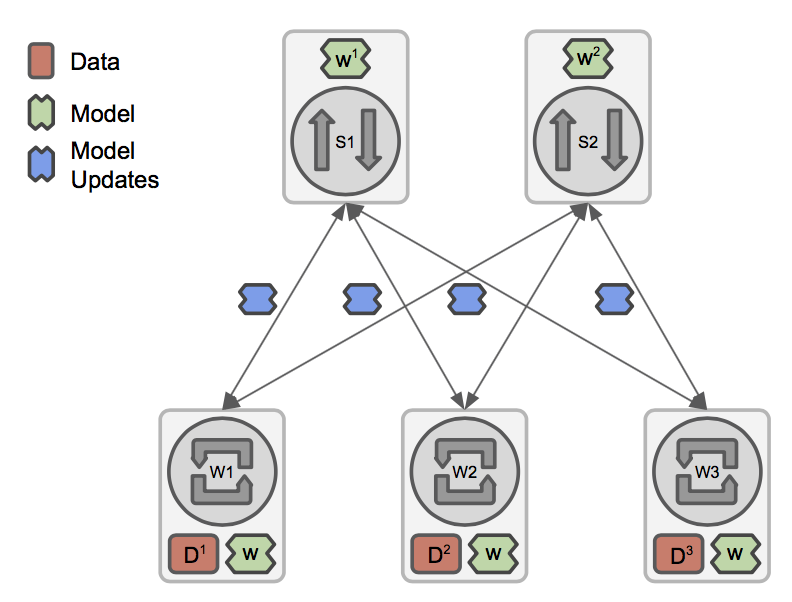
\includegraphics[width=0.4\textwidth]{img/param_server.eps}
\caption{Parameter Server}
\label{fig:param_server}
\end{figure}


\subsection{Consistency}

The most important part of any distributed system is the synchronization strategy used to ensure consistency among multiple nodes concurrently accessing and updating the parameters stored on the parameter server. There are multiple schemes to synchronize nodes during the iterative parameter refinement. \textit{Bulk synchronous parallelization (BSP)} leads to the best algorithm throughput (e.g. convergence achieved over the number of data points processed). Essentially each worker must finish its iteration and push all updates to the parameter server. The server then computes a refined model according to Eq. \ref{eq:bsp_upd} and each node retrieves the updated parameters before beginning the next iteration. This synchronization scheme guarantees consistency among all nodes at all times.
\begin{equation}
W^{t} = W^{(t-1)} + \frac{1}{K}\sum_{k=1}^{K}\Delta(W^{(t-1)}_{k}, D_{k})
\label{eq:bsp_upd}
\end{equation}
While this synchronization strategy essentially recovers the sequential algorithm for a single machine and has the same convergence properties and guarantees, it suffers from a severe limitation when used in a distributed setup \cite{langford2009slow}. Imagine one of the workers is for some reason a lot slower than the others. Due to the synchronization strategy, the other workers have to wait for this particular worker to complete its iteration. This is well known as the straggler problem \cite{ananthanarayanan2013effective} and can seriously affect performance in a distributed environment, because the progress is limited by the slowest node in the cluster.
The second strategy is \textit{total asynchronous parallelization (TAP)}. Similar to BSP, all nodes push their parameter updates to the server after each iteration but in this case, the changes are applied to the model immediately. No waiting for other workers is required, resulting in a very high data throughput. The straggler problem can be mitigated by this synchronization scheme as well, depicted in Figure \ref{fig:workers}. Even though worker 3 is a straggler, the remaining workers can continue with their next iterations without waiting for slower workers. Although this consistency scheme seems to work quite well in practice \cite{li2014scaling}, it lacks formal convergence guarantees and can even diverge \cite{dai2014high}. The reason is that no bound exists for a situation where the divergence in iterations between the slowest and the fastest worker is unbound.
A middle ground between bulk synchronous parallelization and total asynchronous parallelization is \textit{stale synchronous parallel (SSP)} \cite{ho2013more} or \textit{bounded staleness (BS)}. As shown in Figure \ref{fig:bsp_workers}, BSP introduces a maximum delay, or staleness threshold, of $\Delta_{max}$ between the slowest and fastest node. This overcomes the limitation of the TAP approach by introducing a bound on the number of iterations. Formal convergence guarantees can be restored while still maintaining the flexibility of asynchronous parallelization and limiting the straggler problem \cite{cipar2013solving}.
